\section{Introducción}

La Discalculia es una discapacidad de aprendizaje específica que afecta la adquisición de habilidades aritméticas. Aunque la falta de  enseñanza, recursos y la baja inteligencia se han relacionado con la etiología de la discalculia, se sabe actualmente que esta discapacidad del aprendizaje es un trastorno cerebral con una predisposición \href{https://doi.org/10.1016/S0887-8994(00)00258-7}{genética familiar}.

\hfill

Por otra parte, \href{https://doi.org/10.1016/S0896-6273(03)00670-6}{hay estudios} que muestran que una forma de este fenotipo está asociado genéticamente con anomalías tanto funcionales como estructurales del surco intraparietal derecho, llevando esta región un papel fundamental en el desarrollo de las habilidades aritméticas.

\hfill

Tras realizar una búsqueda en “HPO” (Human Phenotype Ontology) del fenotipo a investigar, vemos que se encuentra clasificado como \href{https://hpo.jax.org/app/browse/term/HP:0002442}{HP:0002442} con un total de 13 fenotipos de otras enfermedades asociadas y un total de 24 genes asociados a esta en HPO.

\hfill

Después de la obtención de los genes asociados del fenotipo a través de HPO, introducimos la lista de estos en \href{https://string-db.org}{STRING}, una base de datos biológica y un recurso web de interacciones proteína-proteína conocidas, que nos devuelve la siguiente imagen:

\begin{figure}[]
	\centering
	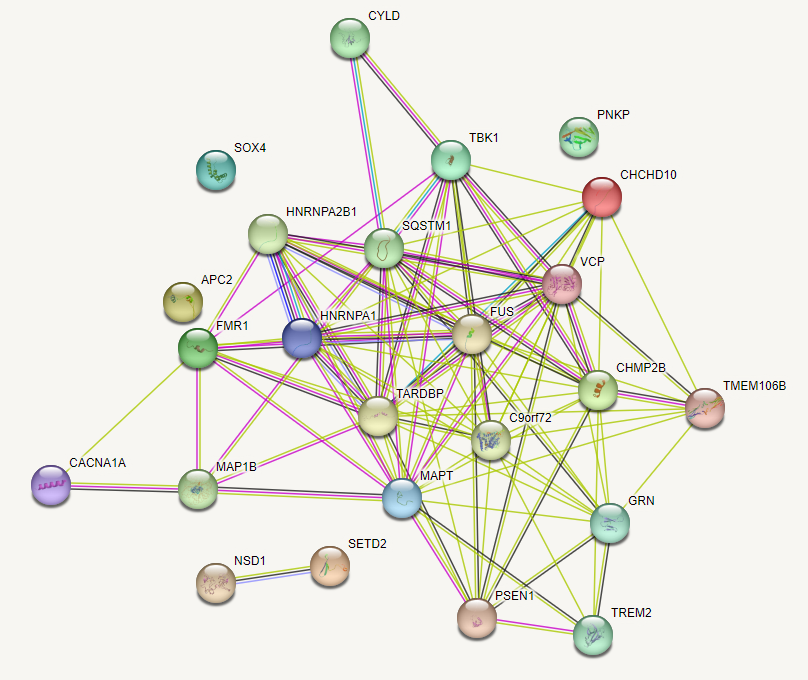
\includegraphics[width=0.50\textwidth]{figures/Gene-Relationships.PNG}
	\caption{Interacciones proteína-proteína a raíz de los genes relacionados. }
	\label{fig:example1}
\end{figure}


\hfill

Tras investigar las distintas interacciones proteína-proteína y observar las enfermedades relacionadas con la discalculia en HPO y los distintos articulos científicos citados anteriormente, la estrecha relación de la discapacidad con un mal funcionamiento del sistema nervioso. En concreto se podría teorizar que existe una relación con las enfermedades de demencia del complejo frontotemporal del cerebro y la esclerosis lateral amiotrófica, pues estas palabras claves aparecen en la mitad de las enfermedades relacionadas con el fenotipo.

\hfill

Enfermedades como Alzheimer u otras que tienen que ver demencias frontotemporales están también fuertemente relacionadas con un número significativo de proteinas relacionadas en la red de interacciones mencionada anteriormente.

\hfill

A raíz de los artículos recomendados por la base de datos \href{https://string-db.org/cgi/network?taskId=bhdt20FXsFkM&sessionId=bx1myVptKrEu}{STRING}, suponemos una relación de estos efectos negativos con una mala conexión entre los hemisferios cerebrales, recordemos que el cerebro delega algunas funciones clave como en este caso puede ser la realización de operaciones matemáticas o el reconocimiento numérico y las interconecta a través del \href{https://es.wikipedia.org/wiki/Cuerpo_calloso}{Cuerpo Calloso}, un mal funcionamiento de este elemento del sistema lleva a una incapacidad de conexión de las funciones de los distintos hemisferios.

\hfill


\hfill

Con estas suposiciones y estas conexiones problema-fallo realizadas, damos comienzo al estudio en profundidad sobre el fenotipo.


